\chapter{Opis projektnog zadatka}
		
		\noindent\textbf{Uvod}\\
		
		\noindent Cilj ovog projekta je razviti \textit{CookBooked}, platformu za zajednicu ljubitelja kuhanja i pečenja kolača, koja omogućava korisnicima razmjenu i otkrivanje recepata iz cijeloga svijeta. Osim toga, platforma treba omogućiti bolje razumijevanje i komunikaciju između korisnika koji dijele istu strast prema kuhanju. Autori recepata će dobiti priliku izgraditi svoju reputaciju, povećati svoju publiku i razmijeniti iskustva s drugima. To će stvoriti motivaciju za kontinuirano stvaranje visokokvalitetnih recepata i sadržaja. S druge strane, korisnici će dobiti priliku unaprijediti vlastite vještine i pričati s autorima recepata te dobiti inspiraciju za vlastite eksperimente u kuhinji. Programska potpora za aplikaciju implementirat će se u obliku web aplikacije.\\
		\begin{figure}[H]
			\centering
			
\includegraphics[width=0.6\textwidth]{slike/CookBooked_logo.png} %veličina u odnosu na 60% širine linije
			\caption{\textit{CookBooked} logo}
			\label{fig:logo} %label mora biti drugaciji za svaku sliku
		\end{figure}
		\eject

		\noindent\textbf{Postojeća slična rješenja}\\

		\noindent Iako postoje mnoge web stranice i aplikacije za dijeljenje recepata, \textit{CookBooked} se izdvaja po svojoj fokusiranosti na interakciju između korisnika. Primjeri postojećih sličnih rješenja uključuju \textit{AllRecipes}, \textit{Tasty} i \textit{Food Network}, no \textit{CookBooked} se razlikuje po svojim značajkama za komunikaciju među korisnicima i praćenje autora.\\
		\begin{figure}[H]
			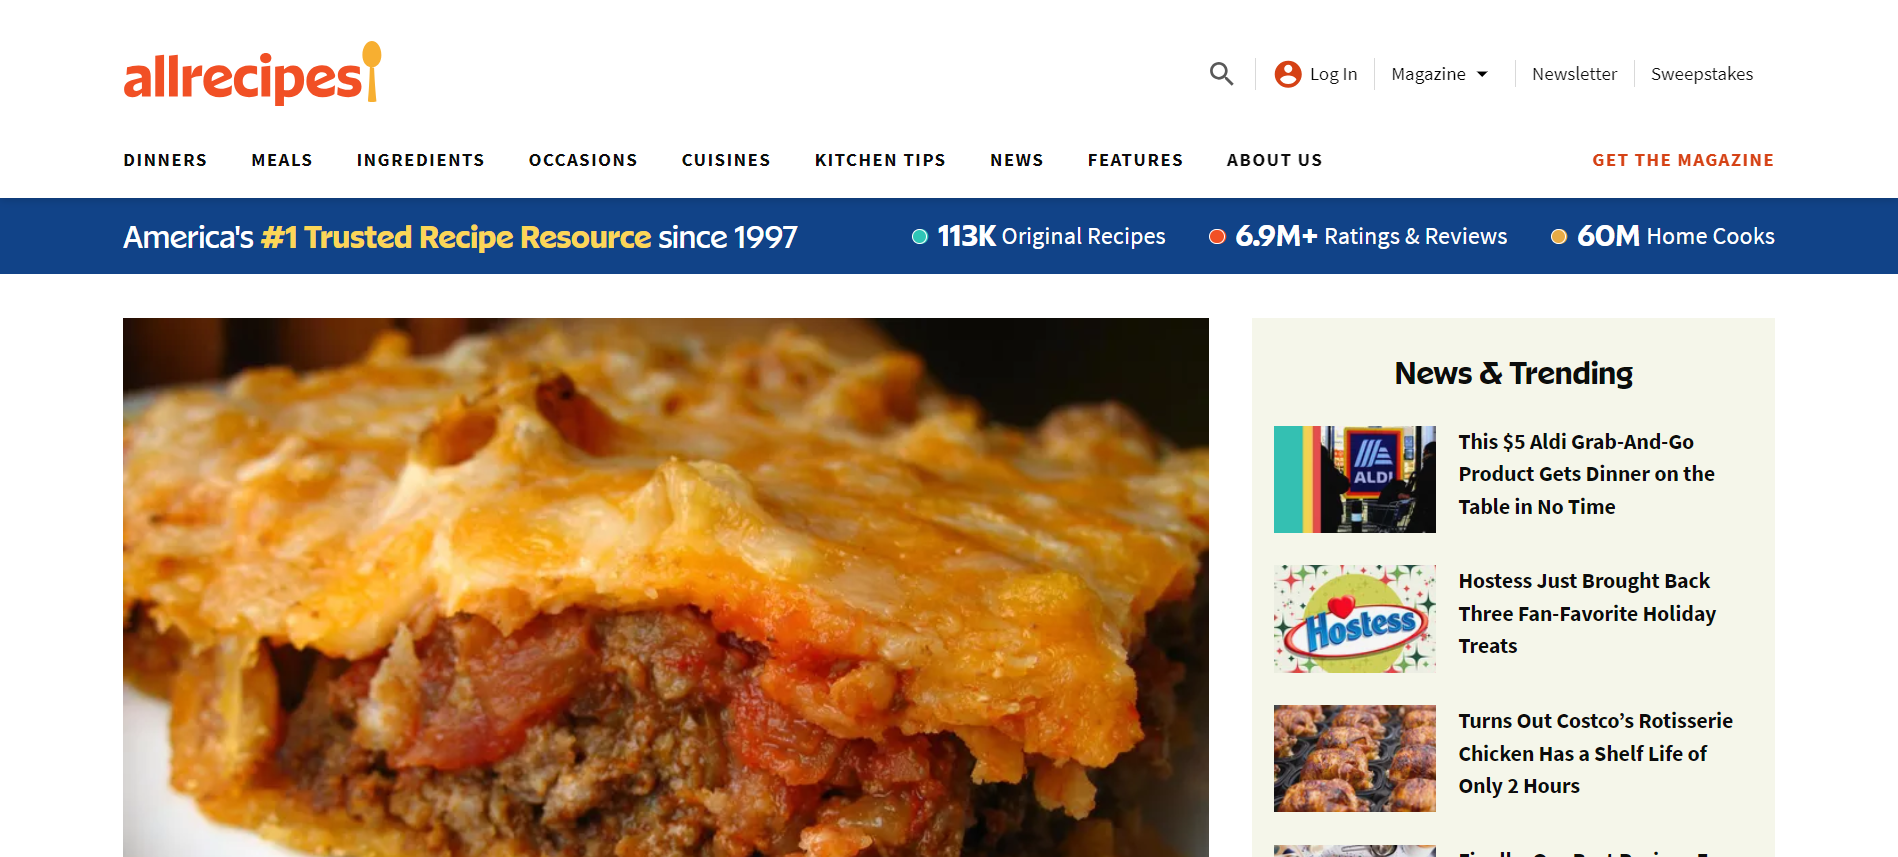
\includegraphics[width=\textwidth]{slike/allrecipes.png}
			\caption{Izgled naslovne stranice \textit{AllRecipes}}
			\label{fig:allrecipes}
		\end{figure}			
		
		\noindent\textbf{Skup korisnika}\\

		\noindent Platformu \textit{CookBooked} može koristiti bilo koji zaljubljenik u hranu i njenu pripremu. Smatramo da će platforma biti najpogodnija ovim skupinama:
		\begin{itemize}
			\item kuhari i ljubitelji kuhanja
			\item osobe s posebnim prehrambenim potrebama (vegetarijanci, vegani, osobe koje ne jedu gluten...)
			\item ljudi koji traže inspiraciju za obroke
			\item autori recepata koji žele podijeliti svoje vještine
		\end{itemize}
		\eject

		\noindent\textbf{Opseg projektnog zadatka}\\

		\noindent Za ostvarenje našeg ambicioznog projekta potrebno je slijedeće:
		\begin{itemize}
			\item razvoj platforme sa svim navedenim funkcionalnostima
			\item stvaranje korisničkog sučelja koje je jednostavno za korištenje
			\item implementaciju sustava za komunikaciju među korisnicima
			\item kreiranje profila za sve tipove korisnika
			\item upravljanje korisnicima i receptima od strane administratora
		\end{itemize}
		\vspace{\baselineskip}
		
		\noindent\textbf{Moguće nadogradnje projektnog zadatka}\\

		\noindent Iako je ovaj projekt unio neke nove ideje i funkcionalnosti u svijet kulinarstva, još uvijek postoje neke nadogradnje i funkcionalnosti koje bi mogle biti implementirane u budućnosti. Neki primjeri nadogradnji su:
		\begin{itemize}
			\item dodavanje dodatnih značajki za napredno pretraživanje recepata
			\item razvijanje mobilne aplikacije za pristup platformi putem mobilnih uređaja
			\item uvođenje funkcionalnosti za online prodaju kuhinjskih proizvoda
			\item integraciju s društvenim mrežama radi širenja korisničke baze
			\item unapređenje sigurnosti i privatnosti podataka korisnika
		\end{itemize}
		\eject